\documentclass[aspectratio=169]{ctexbeamer}
\definecolor{urls}{RGB}{137, 180, 250}
\definecolor{link_text}{RGB}{245, 224, 220}
\hypersetup{
  colorlinks,
  linkcolor=, % This config controls the jumps inside the pdf
  urlcolor=urls,
}
\renewcommand{\UrlFont}{\ttfamily\scriptsize}

\usetheme{AnnArbor}
\usepackage[style=Mocha,accent=Rosewater]{beamercolorthemecatppuccin}

\usefonttheme{serif}
\usefonttheme{professionalfonts}

\usepackage[T1]{fontenc}
\setmainfont{LXGW WenKai}
% \setmainfont{Cascadia Code NF}
% \setsansfont{}
\setmonofont{Cascadia Code NF}
\usepackage{xeCJK}
\setCJKmainfont{LXGW WenKai}
% \setCJKmainfont{}
\setCJKmonofont{Cascadia Code NF}
\newcommand{\nerd}[1]{\texttt{#1}}
\setmonofont{Cascadia Code NF}[
  Contextuals=Alternate
]

\PassOptionsToPackage{hyphens}{url}
% \usepackage{ulem}
\usepackage{graphicx}
%\usepackage{wrapfig}
\usepackage{pifont} % Symbols used as itemize symbols
\usepackage{enumitem}
\setlist[itemize,1]{label={\small\color[RGB]{242, 205, 205}\ding{111}}}
\setlist[itemize,2]{label={\footnotesize\color[RGB]{242, 205, 205}\ding{111}}}
\setlist[itemize,3]{label={\scriptsize\color[RGB]{242, 205, 205}\ding{111}}}
\usepackage{float}
\usepackage{booktabs}

\setbeamerfont{footnote}{size=\tiny}
\setbeamertemplate{footnote}{%
  \color[RGB]{108, 112, 134}%
  \insertfootnotetext%
}
\setlength{\footnotesep}{0.3\baselineskip}
\newcommand{\refnote}[1]{\footnotetext{#1}}

\usetheme{AnnArbor}

\usepackage{amsmath, amssymb, amsthm}
\usepackage{listings}
\lstdefinestyle{bash}{
  alsoletter=-,
  keywordstyle=[2]{\color[RGB]{243, 139, 168}},
  morekeywords=[2]{sudo},
  keywordstyle=[3]{\color[RGB]{166, 227, 161}},
  morekeywords=[3]{add-apt-repository, apt-get, apt},
  keywordstyle=[4]{\color[RGB]{250, 179, 135}},
  morekeywords=[4]{install},
}
\lstdefinestyle{lua}{
  alsoletter=-,
  keywordstyle=[2]{\color[RGB]{137, 180, 250}},
  morekeywords=[2]{name, priority, opts, config, dependencies, submodules, main, version, init, number, boolean, event},
  keywordstyle=[3]{\color[RGB]{180, 190, 254}},
  morekeywords=[3]{fun, setup},
  keywordstyle=[4]{\color[RGB]{250, 179, 135}},
  morekeywords=[4]{},
}
\lstdefinestyle{path}{
  alsoletter=~,
  basicstyle={\footnotesize\ttfamily\color[RGB]{147, 153, 178}\itshape},
}
\lstset{
  language={[5.1]lua},
  style=lua,
  basicstyle=\footnotesize\ttfamily,
  breaklines=true,
  showstringspaces=false,
  breakatwhitespace=true,
  keywordstyle=\color[RGB]{245, 169, 127},
  numberstyle={\ttfamily\color[RGB]{110, 115, 141}},
  commentstyle={\color[RGB]{147, 153, 178}\itshape},
  stringstyle={\color[RGB]{166, 218, 149}},
}
% NOTE: \lstinline{} command does not support background color
\lstdefinestyle{nvim}{
  alsoletter=:,
  keywordstyle=[3]{\color[RGB]{166, 227, 161}},
  morekeywords=[3]{:Tutor, :help, :checkhealth}, % ChkTeX 26
  keywordstyle=[4]{\color[RGB]{250, 179, 135}},
  morekeywords=[4]{snacks},
}

\newcommand{\TODO}[1]{\textcolor{red}{TODO\@: #1} }

% \newcommand{\link}[3][]{\href{#3}{#2}\footnote[#1]{\url{#3}}}
\newcommand{\link}[3][]{\href{#3}{#2\textsuperscript{\nerd{}}}}


\title{Neovim从入门到出门}
\subtitle{第六节:代码格式化、检查与诊断显示}
\author{Jacky-Lzx}
\date{\today}

\usepackage{tikz}
\titlegraphic {
  \begin{tikzpicture}[overlay,remember picture]
    \node at (-6, 4.5){
      
\includegraphics[height=1cm]{./Figures/Neovim_logo.png}
    };
    \node at (6, 4.5){
      
\includegraphics[height=1cm]{./Figures/Catppuccin_logo.png}
    };
  \end{tikzpicture}
}

\usepackage{makecell}

\begin{document}

\begin{frame}
  \titlepage
\end{frame}

\begin{frame}{大纲}
  \tableofcontents
\end{frame}
% Current section
\AtBeginSection[ ] {
  \begin{frame}{大纲}
    \tableofcontents[currentsection]
  \end{frame}
}

\section{本节介绍}

  \begin{frame}{本节介绍}
    \begin{itemize}
      \item \textbf{代码格式化(format)}
        \begin{itemize}
          \item 保存文件时自动格式化代码,使代码符合某种设定的格式规范
          \item 某些语言服务器(LSP)提供该功能
        \end{itemize}
      \item \textbf{代码检查(lint)}
        \begin{itemize}
          \item 在编辑器中实时检查代码的语法错误和潜在问题
          \item 某些LSP提供该功能
        \end{itemize}
      \item \textbf{代码诊断信息显示}
        \begin{itemize}
          \item 显示代码检查和LSP的诊断信息
        \end{itemize}
    \end{itemize}

  \end{frame}

\section{插件安装}

  \subsection{conform.nvim:代码格式化}
    \begin{frame}[fragile]{\link{conform.nvim}{https://github.com/stevearc/conform.nvim}:代码格式化}
      \begin{lstlisting}
  {
    "stevearc/conform.nvim",
    event = "BufWritePre",
    opts = {
      formatters_by_ft = {
        lua = { "stylua" },
        ["_"] = { "trim_whitespace" },
      },
      format_on_save = {
        -- These options will be passed to conform.format()
        timeout_ms = 500,
        lsp_format = "fallback",
      },
    },
  }
      \end{lstlisting}
    \end{frame}

  \subsection{nvim-lint:代码检查}
    \begin{frame}[fragile]{\link{nvim-lint}{https://github.com/mfussenegger/nvim-lint}:代码检查}
      \begin{lstlisting}
  {
    "mfussenegger/nvim-lint",
    event = "BufWritePost",
    config = function()
      vim.api.nvim_create_autocmd({ "BufWritePost" }, {
        callback = function()
          require("lint").try_lint()
          require("lint").try_lint("codespell")
        end,
      })
    end,
  }
      \end{lstlisting}
    \end{frame}

  \subsection{trouble.nvim:代码诊断显示}
    \begin{frame}[fragile]{\link{trouble.nvim}{https://github.com/folke/trouble.nvim}:代码诊断显示}
      \begin{columns}
        \begin{column}{0.3\linewidth}
          \begin{lstlisting}
  {
    "folke/trouble.nvim",
    cmd = "Trouble",
    opts = {},
  }
    \end{lstlisting}
        \end{column}
        \begin{column}{0.7\linewidth}
          \begin{figure}[H]
            \centering
            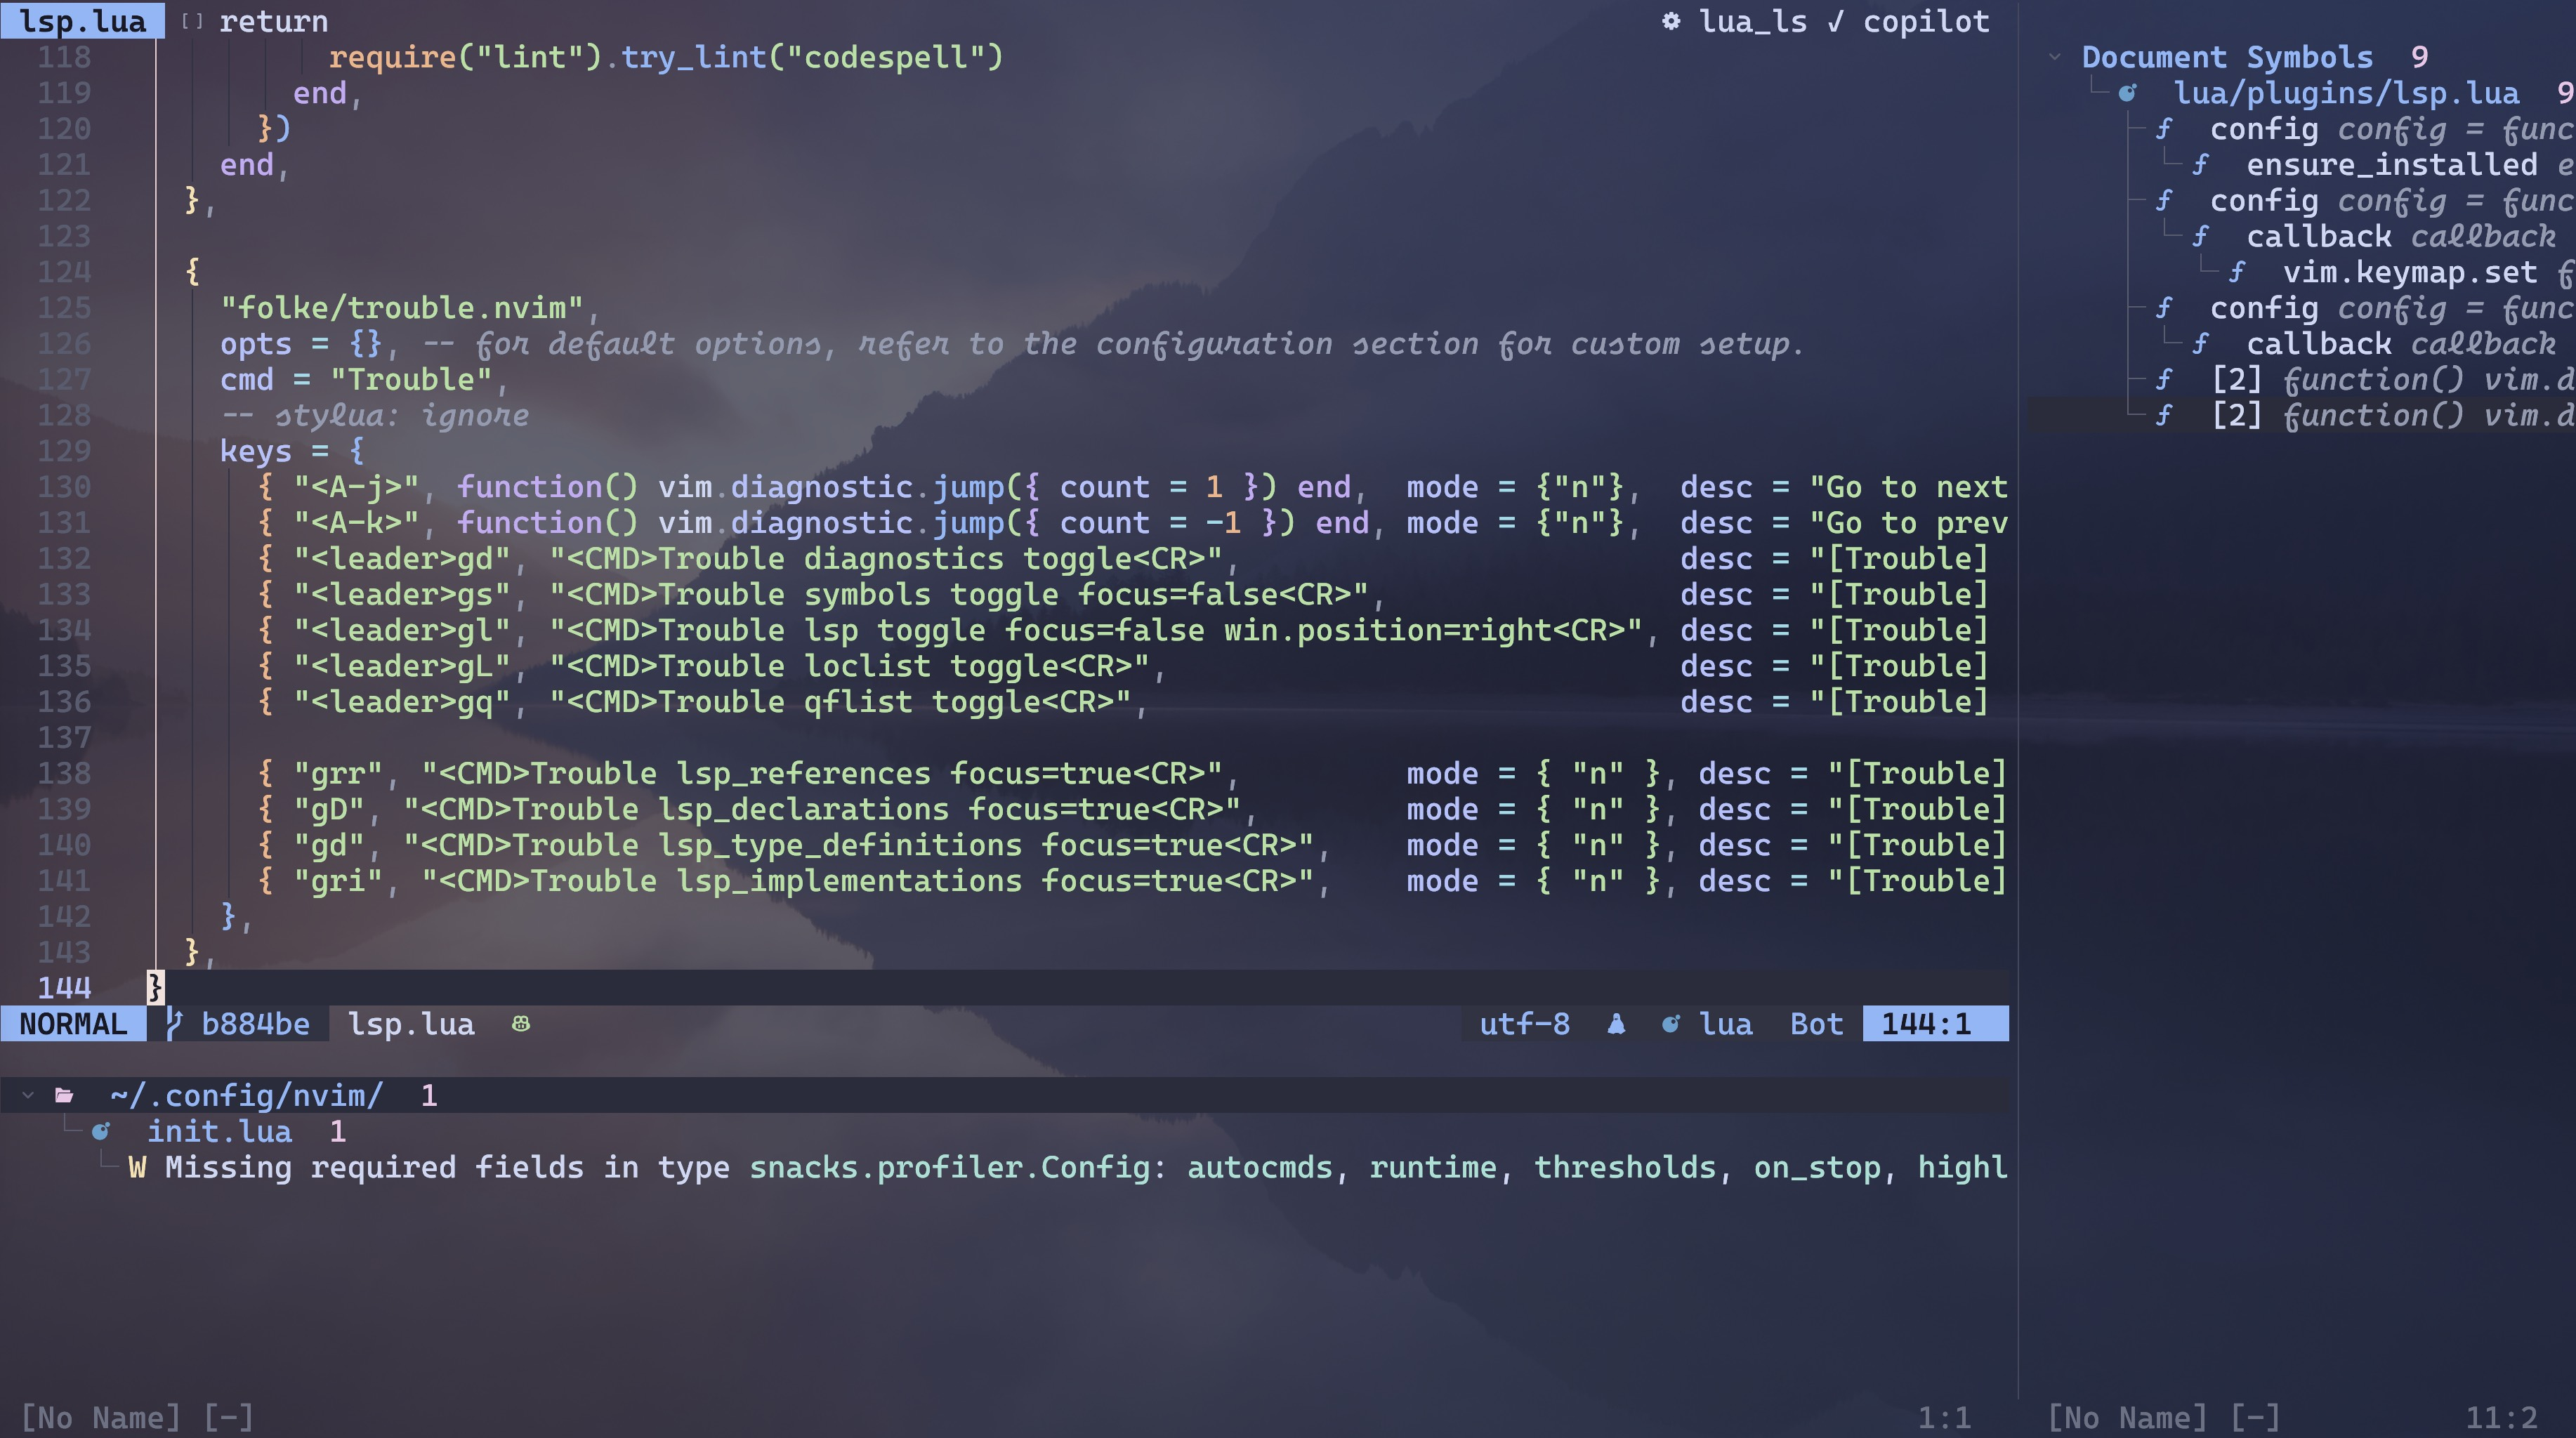
\includegraphics[width=0.9\linewidth]{./Figures/Trouble_UI.jpg}
          \end{figure}
        \end{column}
      \end{columns}
    \end{frame}

\section{插件配置}

  \begin{frame}{插件配置}
    \begin{itemize}
      \item 配置文件目录:\lstinline[language={}, style=path]{\~/.config/nvim/lua/plugins/lsp.lua}
      \item conform.nvim
        \begin{itemize}
          \item 添加lua代码格式化器stylua
          \item 在文件保存时自动格式化代码
          \item 添加启用/禁用自动保存设置
          \item 文件保存时去除行尾空格,取代trim.nvim插件
        \end{itemize}
      \item nvim-lint
        \begin{itemize}
          \item 添加codespell代码检查器,检查拼写错误
        \end{itemize}
      \item trouble.nvim
        \begin{itemize}
          \item 添加快捷键
          \item 添加与LSP的集成
          \item 添加与lualine.nvim的集成
        \end{itemize}
    \end{itemize}

  \end{frame}

  \begin{frame}
    \begin{itemize}
      \item 感谢:
        \begin{itemize}
          \item \link{Catppuccin}{https://catppuccin.com/} 
\includegraphics[height=10pt]{./Figures/Catppuccin_logo.png}
          \item \link{Catppuccin for beamer}{https://github.com/atticus-sullivan/beamercolortheme}
        \end{itemize}
        \vspace{0.5cm}
      \item 本教程的全部材料可以在我的Github上找到
        \begin{itemize}
          \item Slides: \url{https://github.com/Jacky-Lzx/nvim.tutorial.slides}
          \item Config: \url{https://github.com/Jacky-Lzx/nvim.tutorial.config}
        \end{itemize}
    \end{itemize}
  \end{frame}

\end{document}
